\section{Plasma Diagnostics}
\label{sec:diagnostic}


\begin{figure*}[t]
	\centering
	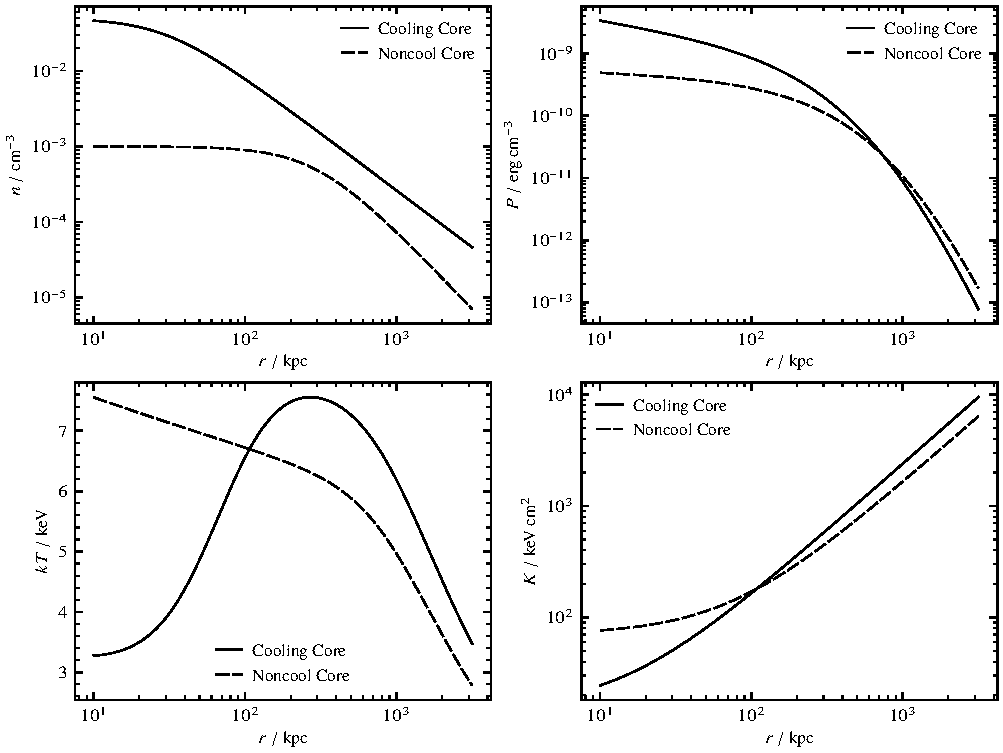
\includegraphics[width=\textwidth, draft=false]{content/theo_profiles.pdf}
	\caption{Theoretical galaxy cluster radial profiles assuming universal selfsimilar scaling relations.
			\textit{Top Left:} Electron number density \cite{vikh2006}. \textit{Top Right:} Gas pressure
			 \cite{arna2010}. \textit{Bottom Left:} Gas temperature \cite{vikh2006}. \textit{Bottom Right:}
			 Gas entropy \cite{cava2009}. Compare to \Cref{fig:chan_profiles} for real observations.}
	\label{fig:theo_profiles}
\end{figure*}


\begin{figure*}[t]
	\centering
	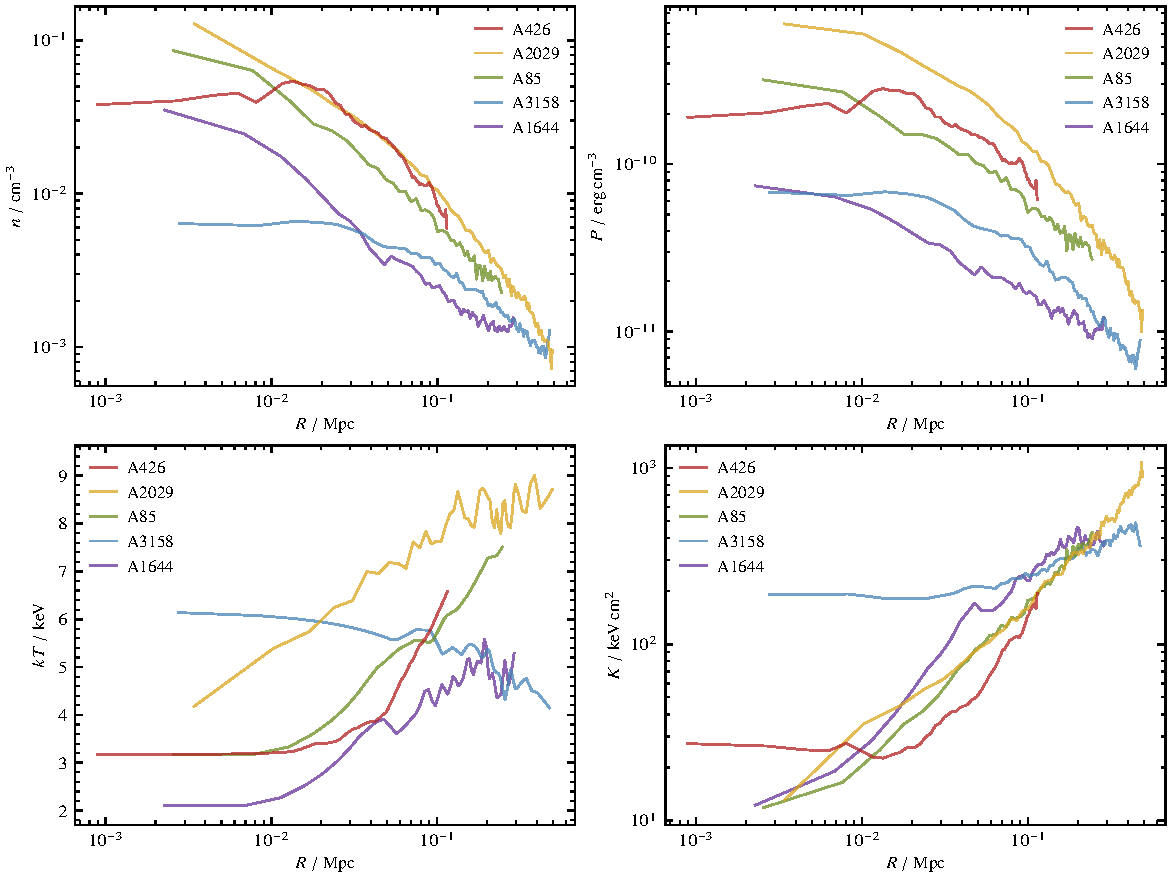
\includegraphics[width=\textwidth, draft=false]{content/chan_profiles.pdf}
	\caption{Sample of galaxy cluster radial profiles from \textit{Chandra} observations \cite{weis2000, cava2009}.
			\textit{Top Left:} Electron number density. \textit{Top Right:} Gas pressure. \textit{Bottom
			 Left:} Gas temperature. \textit{Bottom Right:} Gas entropy. Compare to \Cref{fig:theo_profiles}
			 for a visualization of theoretical and empirical fits with realistic parameter choices.}
	\label{fig:chan_profiles}
\end{figure*}


As a fundamental theoretical baseline, galaxy clusters are modeled as systems governed purely by gravitation. Due to the
scale invariance of gravity, they should then only differ by predictable mathematical scalings that depend solely on mass or
temperature. In reality, Supermassive Black Hole (SMBH) accretion through AGN feedback and cooling in the cluster core disturb
this idealized view. To understand these physics, we compare the deviations of several key ICM properties from our naive
expectation about their behavior.

Most generally, the procedure of how to extract properties from a measured \xray spectrum involves a computational CIE plasma
model fitting the best estimators for temperature, density, abundances and redshift to the given. Perhaps the most famous ones
are the legacy MEKAL and modern APEC codes, which are both implemented in the XSPEC software. Historical observations could
often not resolve the extended ICM and used simpler isothermal models to extract data. As discussed previously, this is at
best a rough approximation and at worst completely inaccurate. Thanks to advances in current \xray telescopes, we have access
to resolved ICM halo datasets from which we can extract radial distributions, although there are still large uncertainties about
nonthermal support from turbulent eddies or bulk movement indicated by hydrodynamical simulations plaguing the field that bias our
results towards lower total masses. Due to the revolution of microcalorimeter spectrographs on board newer missions, it is however
expected that these unknowns will now be solved with higher precision measurements.

To translate our two dimensional images to radial profiles, we need to correct for the projection from three dimensions along the
line of sight to the detector. The basic algorithm do this decomposes our cluster into multiple annuli around the central core.
Starting from the outermost annulus, we fit our spectrum and since there is little pollution from foreground or background layers,
we assume that it represents a uniform shell around the whole system, taken as radially symmetric. Using this, we compute the
corrections which have to be subtracted from the adjacent inner annulus and fit our plasma model to its now cleaned spectrum. By
iteratively peeling layer by layer from the cluster, we deproject our image onto the radius of the system. For CC clusters, this
is usually sufficient, but for some highly disrupted NCC cases, more sophisticated methods are required.

From the employed plasma model, we know the best fitting density $n$ and temperature $T$ parameters. With these, we can simply apply
the ideal gas law
\begin{equation*}
	P = nkT
\end{equation*}
to calculate the pressure. We get
\begin{equation*}
	K = kT / n^{2/3}
\end{equation*}
for the astrophysical entropy. This quantity tracks 

adiabatic... smth


\lipsum[12-20]

\cite{zhan2026}
